
%(BEGIN_QUESTION)
% Copyright 2008, Tony R. Kuphaldt, released under the Creative Commons Attribution License (v 1.0)
% This means you may do almost anything with this work of mine, so long as you give me proper credit

Qualitatively sketch the height/volume relationship for a stepped cylindrical vessel:

$$\includegraphics[width=15.5cm]{i02926x01.eps}$$

\vskip 20pt \vbox{\hrule \hbox{\strut \vrule{} {\bf Suggestions for Socratic discussion} \vrule} \hrule}

\begin{itemize}
\item{} At which point in the vessel's height is the level transmitter's calibration most critical?  In other words, where along the height range will a given height-measurement error translate into the greatest {\it volume} measurement error?
\end{itemize}

\underbar{file i02926}
%(END_QUESTION)





%(BEGIN_ANSWER)

$$\includegraphics[width=15.5cm]{i02926x02.eps}$$

Liquid level instrument calibration is most critical at the wider span of the vessel.

$$\includegraphics[width=15.5cm]{i02926x03.eps}$$

%(END_ANSWER)





%(BEGIN_NOTES)


%INDEX% Measurement, level: characterization for an irregular cylinder

%(END_NOTES)


